
%
%\begin{frame}{Synset induction}
%	\textbf{ACL'17}~\cite{ustalov-panchenko-biemann:2017:Long}
%	
%	
%	%\block{Sample Synsets Induced by the \watset{[MCL, MCL]} Method for English}{
%\vspace{1em}
%Examples of extracted synsets:
%\vspace{1em}
%\centering
%\begin{tabular}{c|p{9cm}}
%\textbf{Size} & \textbf{Synset}\\\hline
%2 & \{\textit{decimal point}, \textit{dot}\}\\
%3 & \{\textit{gullet}, \textit{throat}, \textit{food pipe}\}\\
%4 & \{\textit{microwave meal}, \textit{ready meal}, \textit{TV dinner}, \textit{frozen dinner}\}\\
%5 & \{\textit{objective case}, \textit{accusative case}, \textit{oblique case}, \textit{object case}, \textit{accusative}\}\\
%6 & \{\textit{radio theater}, \textit{dramatized audiobook}, \textit{audio theater}, \textit{radio play}, \textit{radio drama}, \textit{audio play}\}\\
%\end{tabular}
%
%
%	
%	
%\end{frame}
%
%
%\begin{frame}{Synset induction}
%	
%	
%Outline of the 'Watset' method:
%
%\vspace{2em}
%
%\centering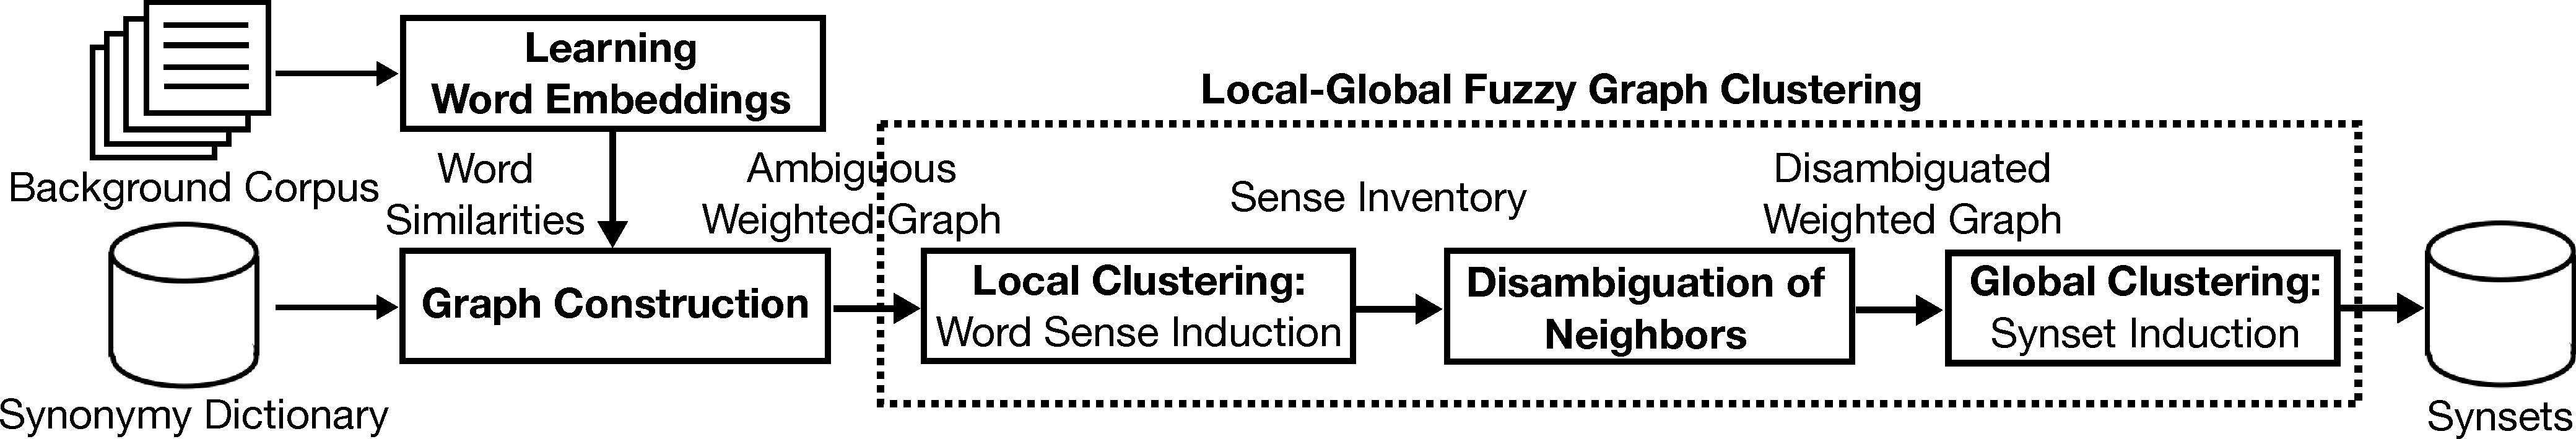
\includegraphics[width=1.05\textwidth]{figures/outline}
%	
%\end{frame}
%
%
%\begin{frame}{Synset induction}
%\centering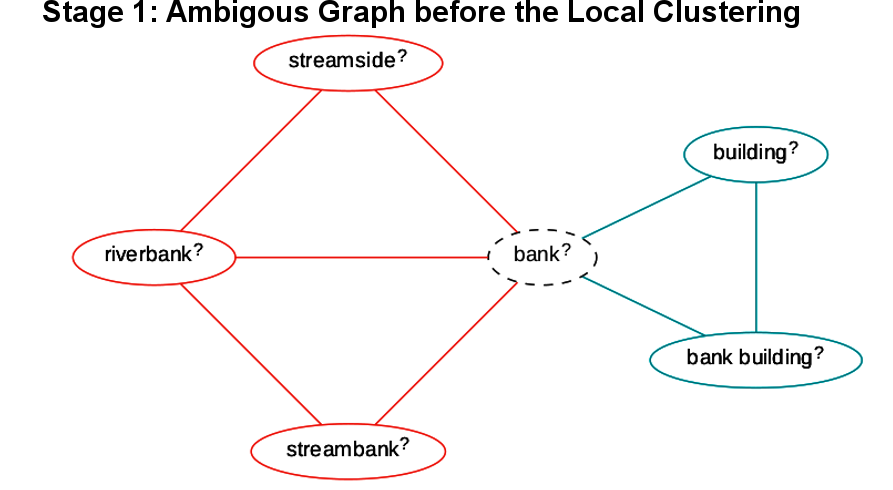
\includegraphics[width=1\textwidth]{figures/stages1}	
%\end{frame}
%
%
%
%\begin{frame}{Synset induction}
%\centering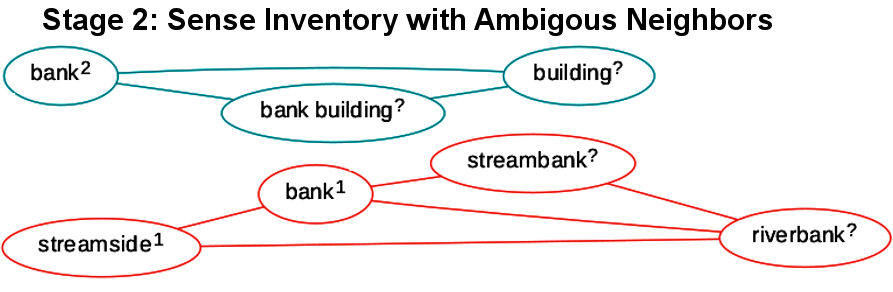
\includegraphics[width=1\textwidth]{figures/stages2}	
%\end{frame}
%
%
%
%\begin{frame}{Synset induction}
%\centering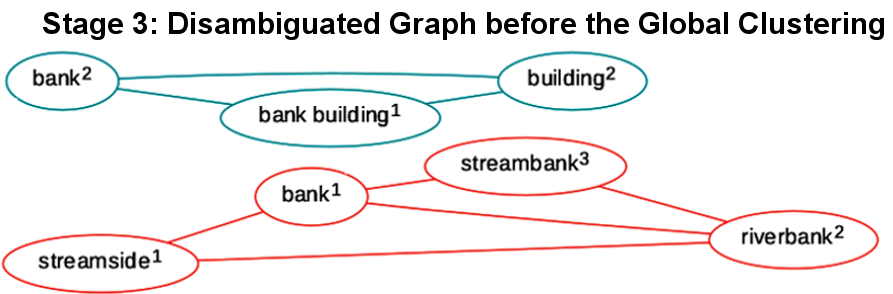
\includegraphics[width=1\textwidth]{figures/stages3}	
%\end{frame}
%
%
%\begin{frame}{Synset induction}
%
%  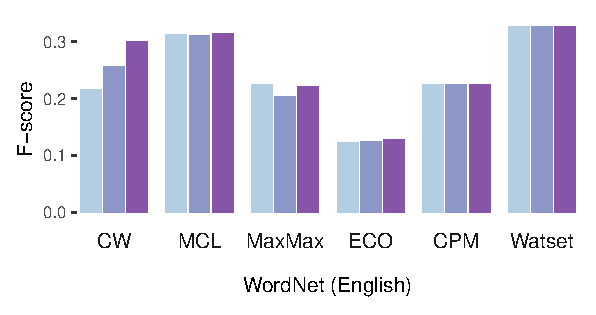
\includegraphics[width=0.49\textwidth]{figures/edges-en-wordnet}  
%  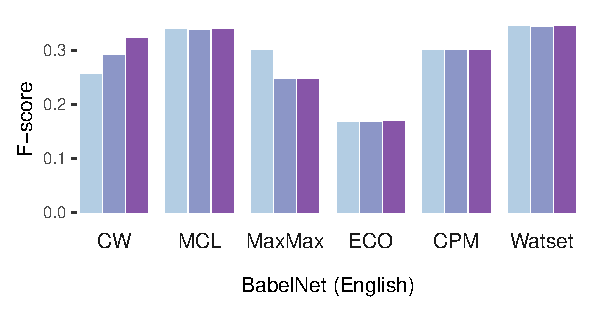
\includegraphics[width=0.49\textwidth]{figures/edges-en-babelnet}
%
%  \pause    
%  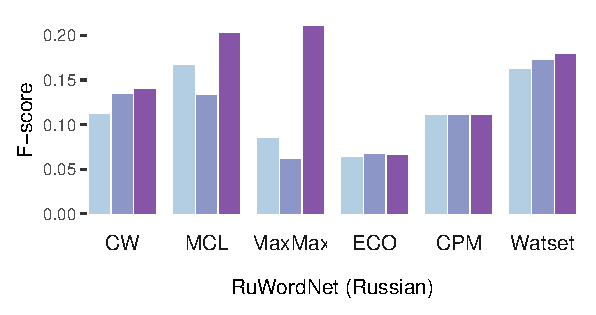
\includegraphics[width=0.49\textwidth]{figures/edges-ru-rwn}     
%  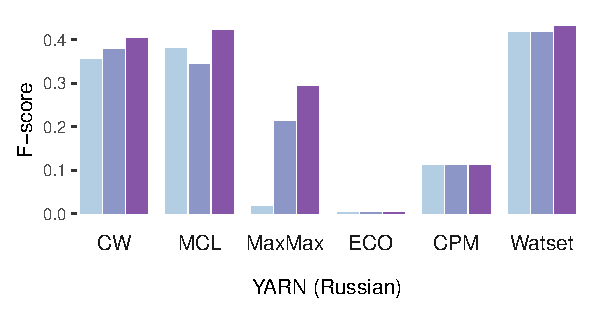
\includegraphics[width=0.49\textwidth]{figures/edges-ru-yarn}     
%	
%\end{frame}
%




\begin{frame}{Semantic roles  }

\begin{itemize}
\item Semantic frame ``Abandonment'' from FrameNet 	
\end{itemize}


	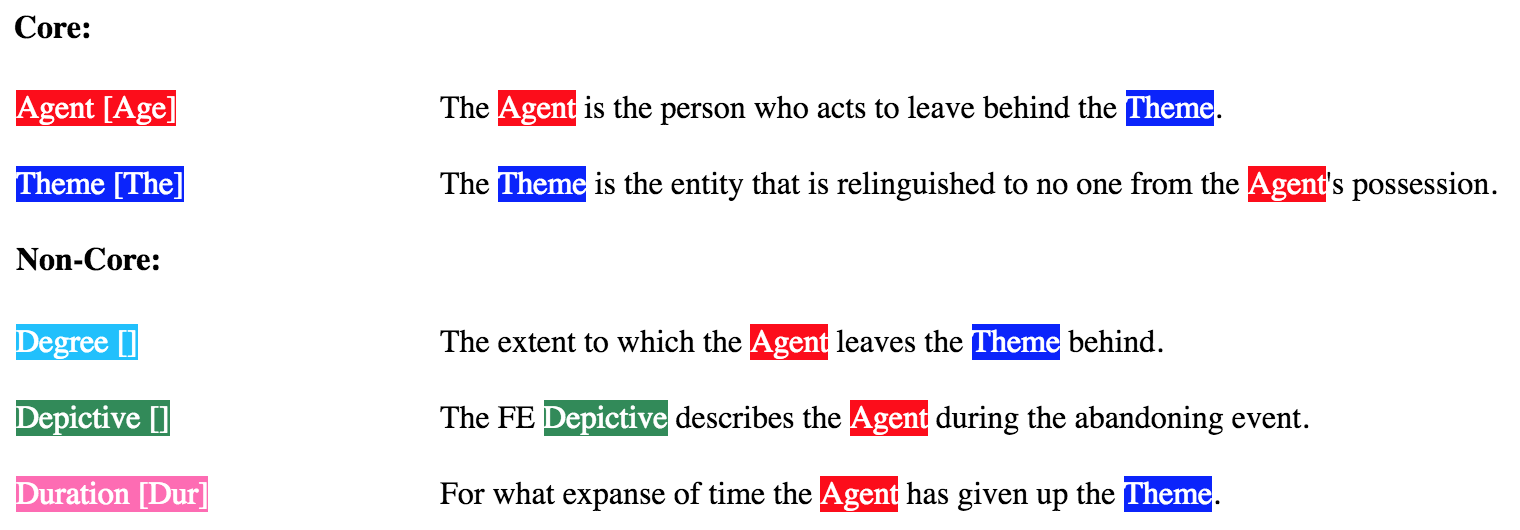
\includegraphics[width=1.0\textwidth]{figures/roles}
\end{frame}



\begin{frame}{Semantic classes  }

\begin{itemize}
\item A semantic class contains words that share a \textbf{semantic feature}.
\item Examples of \textbf{concrete semantic classes}:
\begin{itemize}
\item  people
\item  plants
\item  animals
\item  materials
\item  programming languages
\end{itemize}

\item Examples of \textbf{abstract semantic classes}: 

\begin{itemize}
\item qualities
\item actions
\item processes
\end{itemize}


  	
\end{itemize}


\end{frame}


	
\begin{frame}{Sample of induced \alert{sense inventory}}


\begin{table}
\centering
\scriptsize
\begin{tabular}{l|p{6cm}|p{2.5cm}} 
\bf Word Sense & \bf Local Sense Cluster: Related Senses & \bf Hypernyms \\
\toprule
 \alert{mango\#0} &  peach\#1, grape\#0, plum\#0, apple\#0, apricot\#0, watermelon\#1, banana\#1, coconut\#0, pear\#0, fig\#0, melon\#0,  \alert{\textbf{mangosteen\#0}}, ... & fruit\#0, food\#0, ... \\
 
\midrule
\alert{apple\#0} & mango\#0, pineapple\#0, banana\#1, melon\#0, grape\#0, peach\#1, watermelon\#1, apricot\#0, cranberry\#0, pumpkin\#0, \alert{\textbf{mangosteen\#0}}, ... & fruit\#0, crop\#0,  ... \\

\midrule
Java\#1 & C\#4, Python\#3, Apache\#3, Ruby\#6, Flash\#1, C++\#0, SQL\#0, ASP\#2, Visual Basic\#1, CSS\#0, Delphi\#2, MySQL\#0, Excel\#0, Pascal\#0, ... & programming language\#3, language\#0, ... \\

\midrule
Python\#3 & PHP\#0, Pascal\#0, Java\#1, SQL\#0, Visual Basic\#1, C++\#0, JavaScript\#0, Apache\#3, Haskell\#5, .NET\#1, C\#4, SQL Server\#0, ... & language\#0, technology\#0, ... \\

\end{tabular}


\end{table}


\note{ entries  representing ``fruits'' and ``programming language'' senses. Each word sense $s$ is represented with a list of related senses $\mathcal{N}(s)$ and the list of hypernyms $\mathcal{H}(s)$. The hypernyms can be used as human-interpretable sense labels of the sense clusters. One sense $s$, such as ``apple\#0'', can appear in multiple entries.}

\end{frame}


\begin{frame}{Sample of induced \alert{semantic classes}}


\begin{table}
\centering
\scriptsize
\begin{tabular}{l|p{2.5in}|p{1in}} 
\bf ID &  \bf Global Sense Cluster: Semantic Class & \bf Hypernyms \\ 

\toprule

1 & peach\#1, banana\#1, pineapple\#0, berry\#0, blackberry\#0, grapefruit\#0, strawberry\#0, blueberry\#0, \alert{mango\#0}, grape\#0, melon\#0, orange\#0, pear\#0, plum\#0, raspberry\#0, watermelon\#0, \alert{apple\#0}, apricot\#0, watermelon\#0, pumpkin\#0, berry\#0, \alert{\textbf{mangosteen\#0}}, ...  & vegetable\#0, fruit\#0, crop\#0, ingredient\#0, food\#0, $\cdot$ \\ 

\midrule

2  & C\#4, Basic\#2, Haskell\#5, Flash\#1, \alert{Java\#1}, Pascal\#0, Ruby\#6, PHP\#0, Ada\#1, Oracle\#3, \alert{Python\#3}, Apache\#3, Visual Basic\#1, ASP\#2, Delphi\#2, SQL Server\#0, CSS\#0, AJAX\#0, JavaScript\#0, SQL Server\#0, Apache\#3, Delphi\#2, Haskell\#5, .NET\#1, CSS\#0, ... & programming language\#3, technology\#0, language\#0, format\#2, app\#0
\end{tabular}

\note{Sample of the induced  sense clusters representing ``fruits'' and ``programming language'' semantic classes. Similarly to the induced word senses, the semantic classes are labeled with hypernyms. In contrast to the induced word senses, which represent a local clustering of word senses (related to a given word) semantic classes represent a global sense clustering of word senses. One sense $c$, such as ``apple\#0'', can appear only in a single cluster.}


\end{table}

\end{frame}


%
%\begin{frame}{Induction of  semantic classes}
%
%Examples of semantic classes:
%
%\begin{table}[ht]
%\centering
%\scriptsize
%\begin{tabular}{l|p{6cm}|p{3.5cm}} 
%
%\bf ID &  \bf Sense Cluster & \bf Hypernyms \\ \hline
%& &  \\
%1 & peach\#1, banana\#1, pineapple\#0, berry\#0, blackberry\#0, grapefruit\#0, strawberry\#0, blueberry\#0, grape\#0, melon\#0, orange\#0, pear\#0, plum\#0, raspberry\#0, watermelon\#0, apple\#0, apricot\#0, ...  &  fruit\#0, crop\#0, ingredient\#0, food\#0, $\cdot$ \\ & &  \\ \hline
%& &  \\
%2  & C\#4, Basic\#2, Haskell\#5, Flash\#1, Java\#1, Pascal\#0, Ruby\#6, PHP\#0, Ada\#1, Oracle\#3, Python\#3, Apache\#3, Visual Basic\#1, ASP\#2, Delphi\#2, SQL Server\#0, CSS\#0, AJAX\#0, the Java\#0, ... & programming language\#3, technology\#0, language\#0, format\#2, app\#0 
%\end{tabular}
%\end{table}
%
%	
%\end{frame}



\begin{frame}{Induction of  semantic classes}
	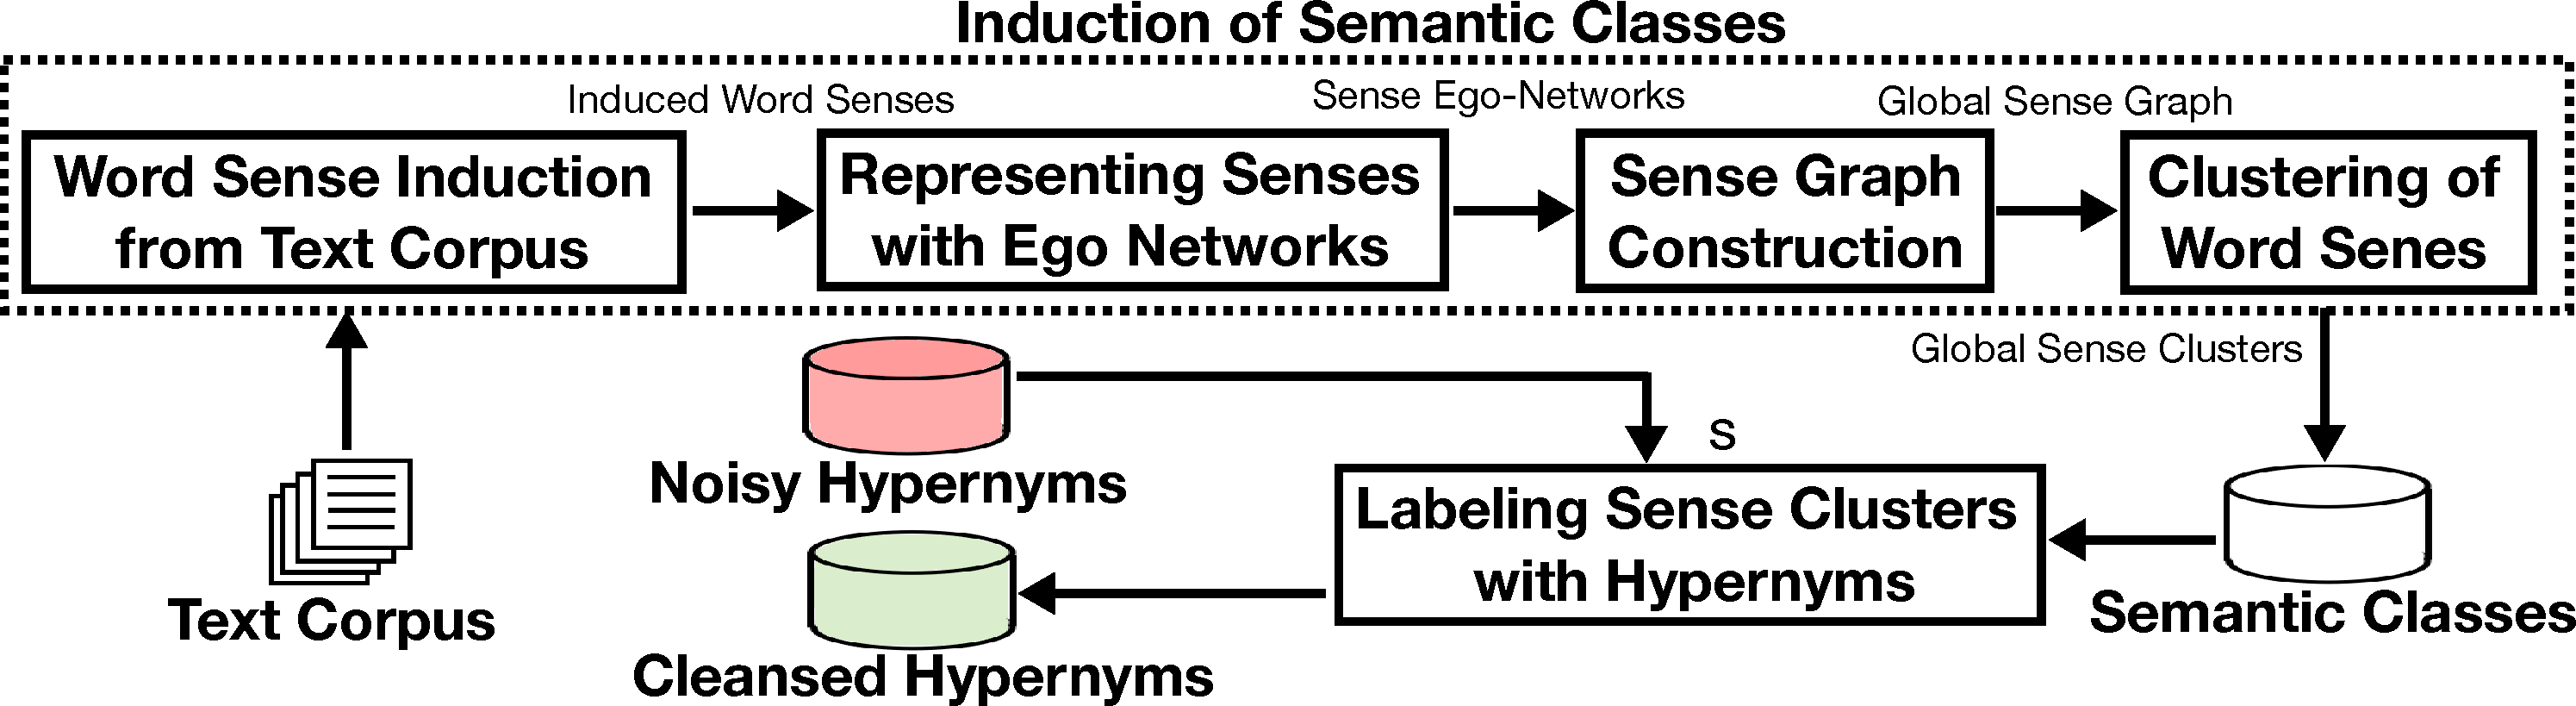
\includegraphics[width=1.0\textwidth]{figures/outline-semantic-classes}
\end{frame}




\begin{frame}{Induction of sense semantic classes}

Filtering noisy hypernyms with semantic classes \textbf{LREC'18}~\cite{panchenko:2018:SemanticClasses}: 

	\centering 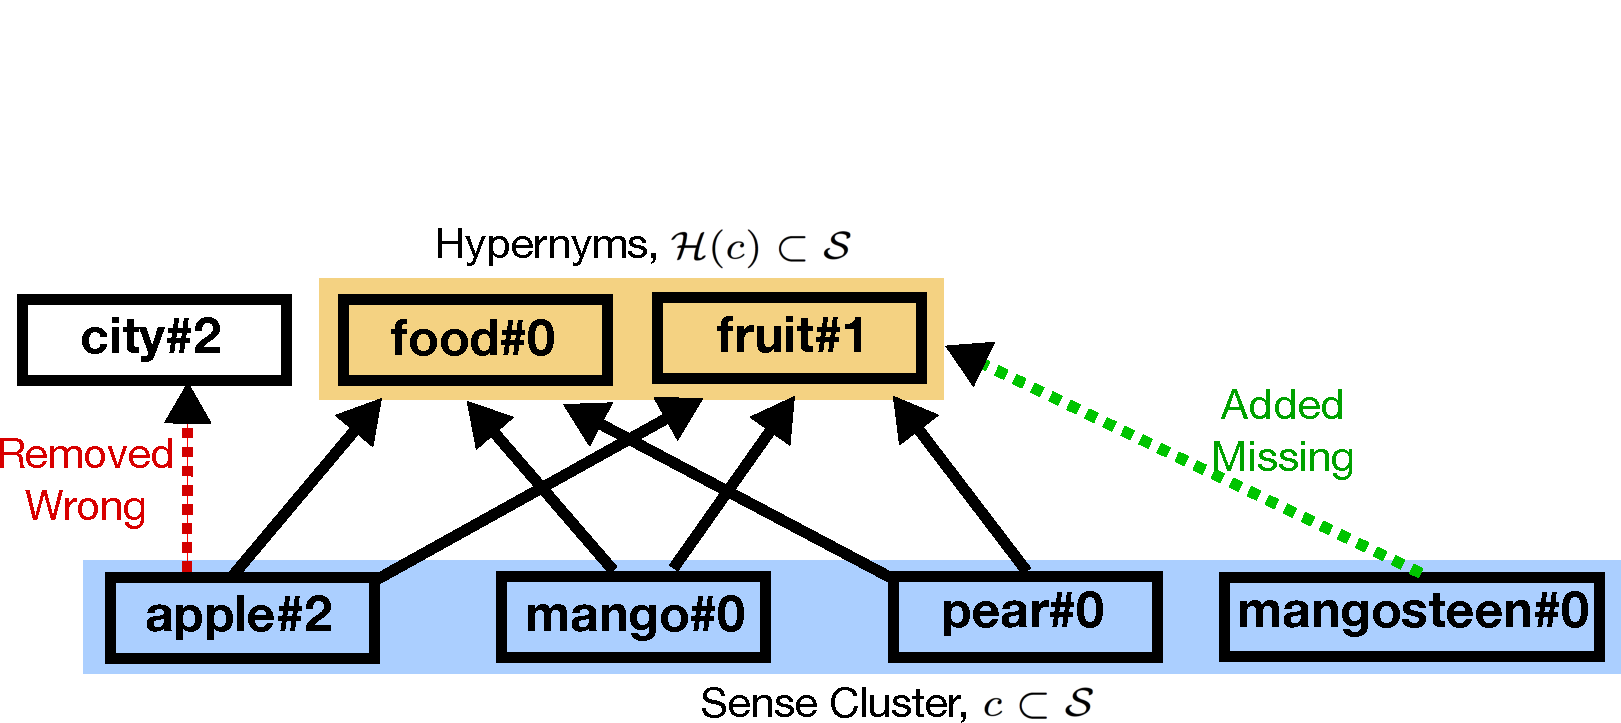
\includegraphics[width=1.0\textwidth]{figures/coset}
	
\end{frame}



\begin{frame}{Global sense clustering}


\vspace{-10pt}
{\footnotesize \underline{\url{http://panchenko.me/data/joint/nodes20000-layers7}}}


\begin{center}
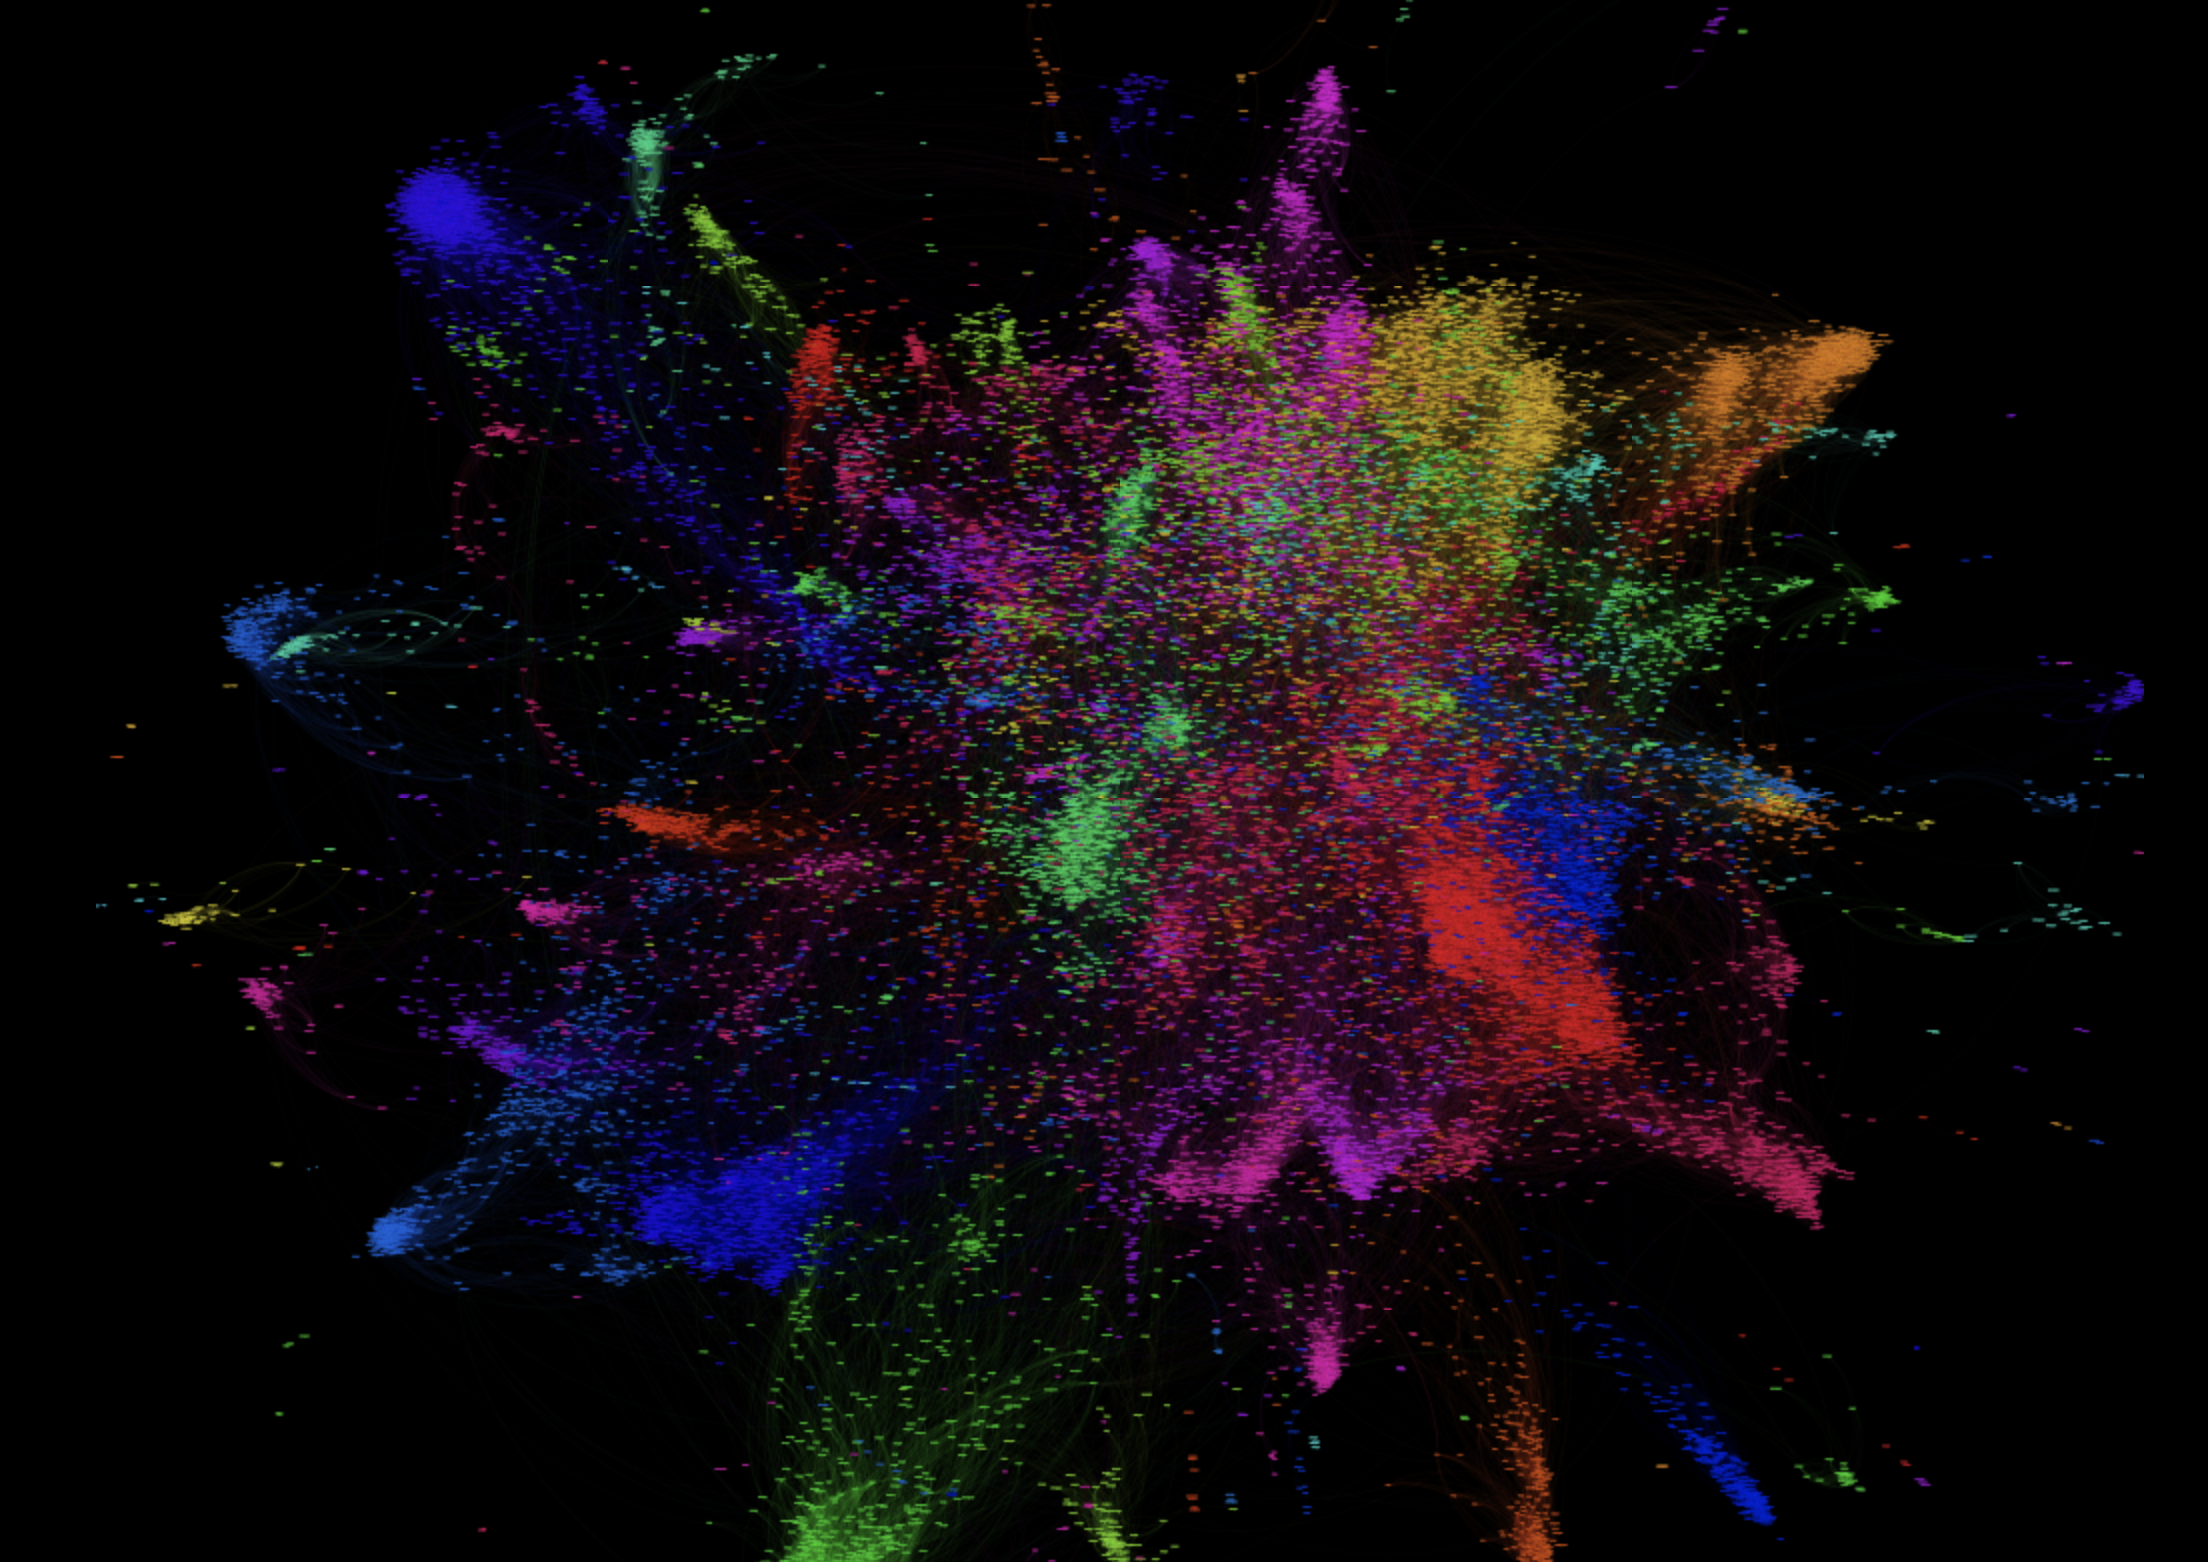
\includegraphics[width=.75\textwidth]{figures/structure}
\end{center}

\end{frame}



\begin{frame}{Global sense clustering}

\begin{center}
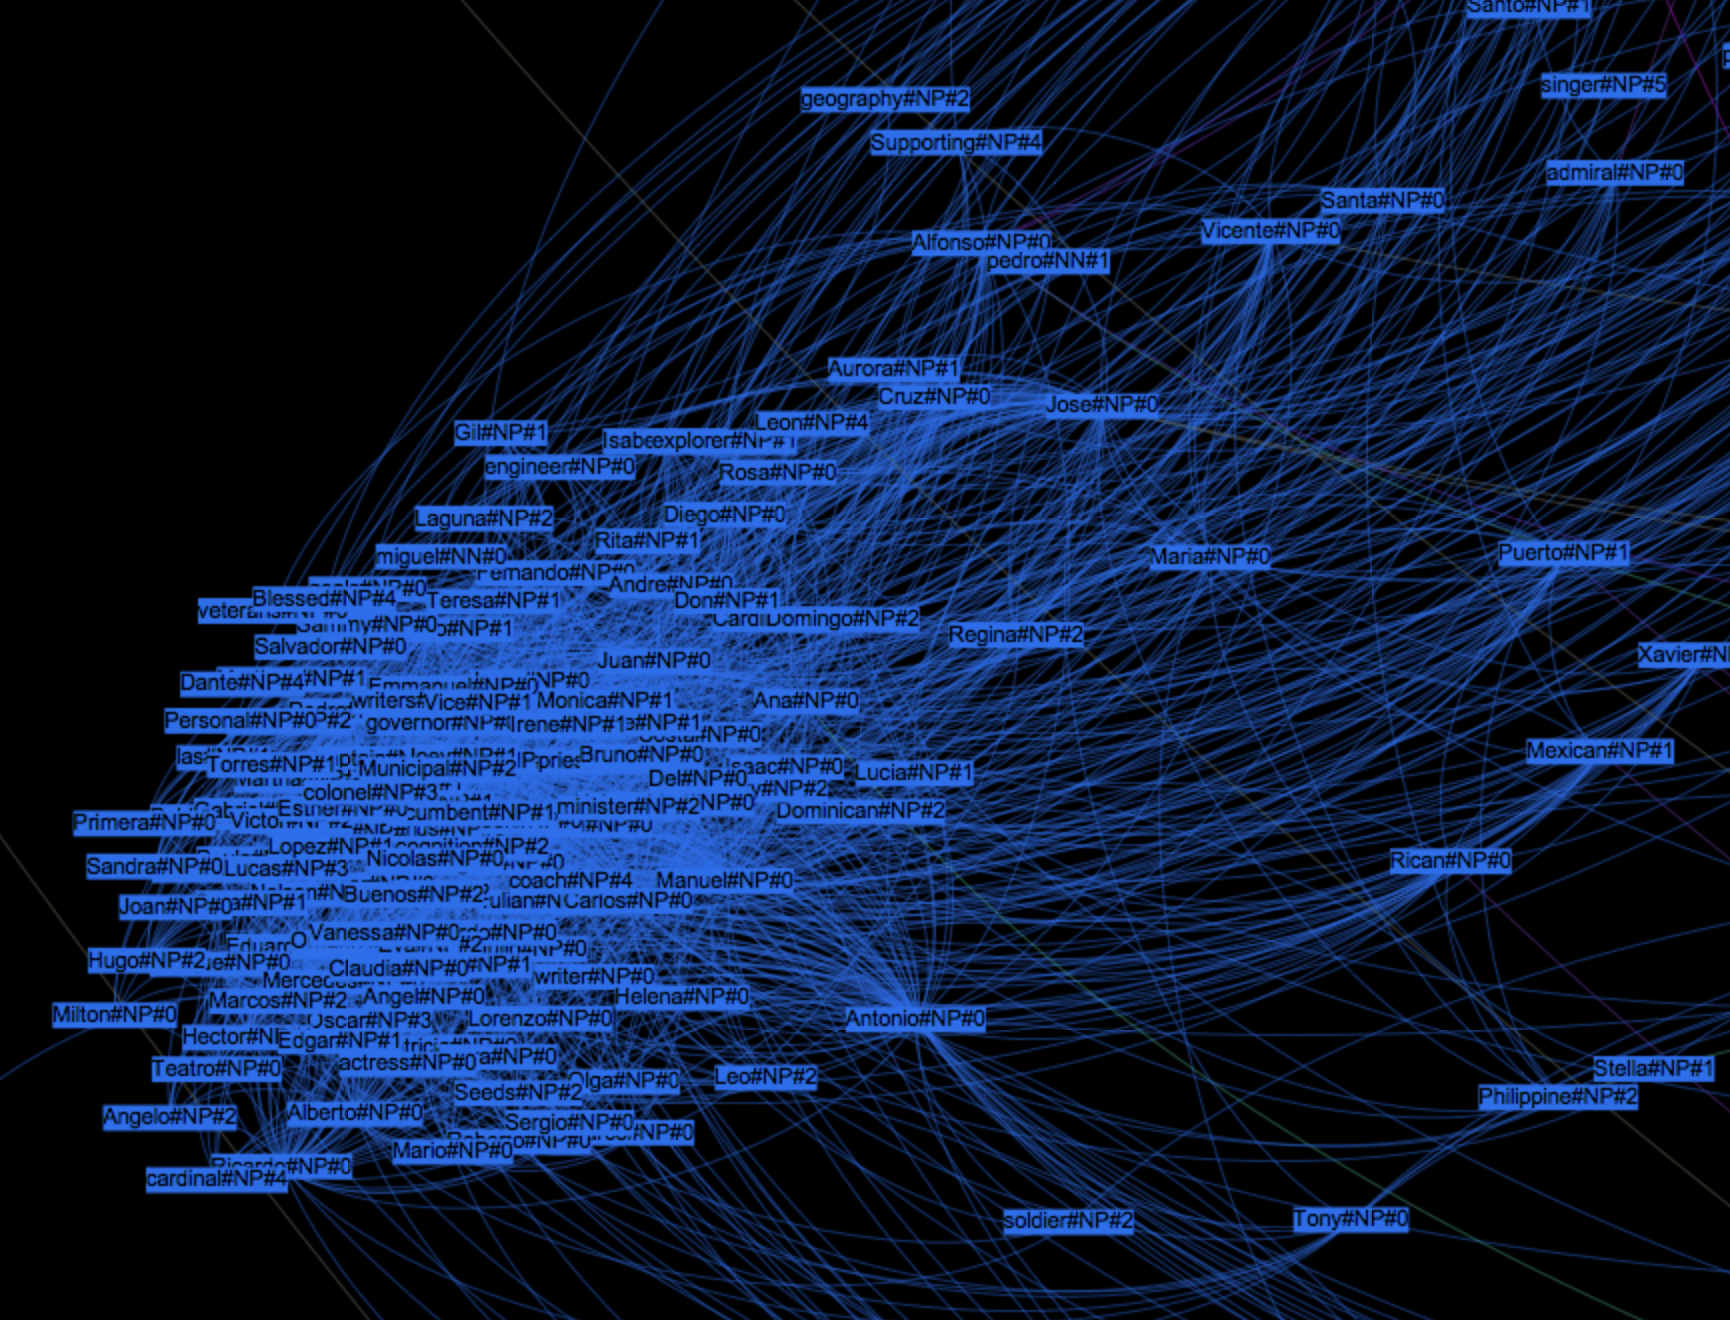
\includegraphics[width=.75\textwidth]{figures/structure1}
\end{center}

\end{frame}



\begin{frame}{Induction of sense semantic classes}

Filtering of a noisy hypernymy database with semantic classes.  \textbf{LREC'18}~\cite{panchenko:2018:SemanticClasses}

\begin{table}
\scriptsize
\centering
\resizebox{1.0\linewidth}{!}{
\begin{tabular}{l|c|c|c}
 & \textbf{Precision} & \textbf{Recall} & \textbf{F-score} \\ \hline
Original Hypernyms  (Seitner et al., 2016) & $0.475$ & $0.546$ & $0.508$ \\
Semantic Classes (coarse-grained) & $\mathbf{0.541}$ & $\mathbf{0.679}$ & $\mathbf{0.602}$ \\
\end{tabular}
}
\end{table}
	
\end{frame}




